\documentclass[10pt,twocolumn,twoside]{IEEEtran}
\usepackage{amsmath}
\usepackage{amsthm}
\usepackage{amsfonts}
\usepackage{amssymb}
\usepackage{bm}
\usepackage[margin=0.8in]{geometry}
\usepackage{mathrsfs}
\usepackage{graphicx}
\usepackage{cite}
\usepackage{epstopdf}
\epstopdfsetup{outdir=./}
\DeclareMathOperator*{\argmin}{arg\,min}
\DeclareMathOperator*{\argmax}{arg\,max}
\newtheorem{definition}{Definition}
\newtheorem{lemma}{Lemma}
\newtheorem{theorem}{Theorem}
\newtheorem{problem}{Problem}
\usepackage{algorithm}
\usepackage{algpseudocode}
\newcommand{\vv}[1]{\mbox{\boldmath $#1$}}
\newcommand{\norm}[1]{\left|\left|#1\right|\right|_2}
\newcommand{\showuc}[1]{\MakeUppercase{#1}}
\algrenewcommand\alglinenumber[1]{\scriptsize #1}
\def \ETx {\mathcal{E}}
\def \TRx {\mathcal{R}}	
\makeatletter
\let\OldStatex\Statex
\renewcommand{\Statex}[1][3]{%
  \setlength\@tempdima{\algorithmicindent}%
  \OldStatex\hskip\dimexpr#1\@tempdima\relax}
\makeatother
\algdef{SE}[DOWHILE]{Do}{DoWhile}{\algorithmicdo}[1]{\algorithmicwhile\ #1}
\title{}

\author{
\thanks{}
}

\begin{document}
\maketitle
\thispagestyle{empty}
\pagestyle{empty}
\begin{abstract}
\end{abstract}


\begin{IEEEkeywords}
\end{IEEEkeywords}

\section{Notations}
% !TEX root = main.tex
The transmitter energy arrival instants are marked by $t_i$'s with energy $\ETx_i$'s for $i \in \{0,1,..\}$. The transmitter has $\ETx_0$ amount of energy at time $t_0=0$. The total energy harvested at the transmitter till time $t$ is given by $\ETx(t)=\sum\limits_{i:t_i < t}\ETx(t)$. Note that $\ETx(t)$ is a staircase like function.
 
The receiver spends a constant $P_{r}$ amount of power to be in `\textit{on}' state during which it can receive data from the transmitter. When it is in `\textit{off}' state it cannot receive data, and uses no power. Hence each energy arrival (say of amount $E$) at the receiver can be viewed as adding $\TRx_i=\dfrac{E}{P_{r}}$ amount of time for which the receiver can be \textit{on}. The instances of energy arrival (which can also be thought of as `\textit{time}' arrivals) at the receiver are denoted by $r_i$. Note that transmitter can only send bits if and only if receiver is \textit{on}. The maximum amount of time for which the receiver (and hence the transmitter) can be \textit{on} assuming no energy arrives at the receiver after time '$t$' is given by the function $\TRx(t)=\sum\limits_{i:t_i\leq t} \TRx_i$.

The rate at which bits are transmitted with power `$p$' is given by function $g(p)$. The function $g(.)$ is assumed to possess the following properties. 
\begin{align}
&P1) &&g(0)=0\text{ and }\lim_{x\rightarrow \infty} g(x)= \infty,\label{property_0_infty}
\\
&P2) &&g(x)\text{ is concave in nature with } x,\label{property_concave}
\\
&P3) &&g(x)\text{ is monotonically increasing with } x,\label{property_increasing}
\\ 
&P4) &&\frac{g(x)}{x} \text{ is convex, monotonically decreasing} \nonumber
\\
&    &&\text{ with } x \text{ and } \lim_{x\rightarrow \infty} \frac{g(x)}{x}= 0.\label{property_decreasing}
\end{align}

%Any policy used for transmission is represented in form of $\{\bm{p},\bm{s},N\}$, where $N\in \mathbb{N}$, $\bm{p}=[p_1\ p_2\ ..\ p_N]$ and $\bm{s}=[s_1\ s_2\ ..\ s_{N+1}]$. The transmitter starts transmitting at time instant $s_1$ with power $p_1$ and continues till time $s_2$. From $s_2$ it transmits with power $p_2$ and so on. The policy ends at time $s_{N+1}$. 

Suppose in a transmission policy, the transmitter starts transmitting at time $s_1$ with power $p_1$ and continues till $s_2$. From $s_2$ it transmits with power $p_2$ and so on. In general, $p_i$ is the power of transmission from $s_i$ to $s_{i+1}$. The last section of transmission begins at time $s_N$ with power $p_N$, where $N\in \mathbb{N}$. The transmission ends at time $s_{N+1}$. The transmitter cannot transmit any bits when the receiver is \textit{off}. Therefore, the receiver is kept \textit{on} when transmitter transmits any bits i.e it is kept \textit{on} during the time $[s_i,s_{i+1}]$ when $p_i > 0$, $\forall \ i=1,2..,N$, and kept \textit{off} when $p_i=0$. Such a policy, sometimes referred to in this paper by the alphabets $X,Y,Z$ or $W$, is represented by the vectors $\bm{p}$, $\bm{s}$ and a number $N$, where $\bm{p}=\{p_1, p_2, .., p_N\}$ and $\bm{s}=\{s_1, s_2, .., s_{N+1}\}$. The total time for which the receiver is \textit{on} is referred to as `transmission time' or `transmission duration' and the time by which the policy get over, is called as the `finish time'. The energy used by this policy at the transmitter upto time `$t$' is given by the function $U(t)$, and the number of bits sent by time $t$ is represented by $B(t)$. Clearly,

%Such a policy is represented by the notation $\{\bm{p},\bm{s},N\}$, where $\bm{p}=\{p_1, p_2, .., p_N\}$ and $\bm{s}=\{s_1, s_2, .., s_{N+1}\}$. The energy used by this policy at the transmitter upto time '$t$' is given by the function $U(t)$ and the bits sent is represented by $B(t)$. Clearly,
\begin{align}
&U(t)=\sum_{i=1}^{j} p_i(s_{i+1}-s_i)+p_{j+1}(t-s_j) \text{ and }
\\
&B(t)=\sum_{i=1}^{j} g(p_i)(s_{i+1}-s_i)+g(p_{j+1})(t-s_j),
\\
&\text{where }j=\argmax_{i} \hspace{2mm}\{(t_i<t)\}.\nonumber
\end{align}
The function $\mathcal{P}(a,b)=\dfrac{\mathcal{E}(b^- )-U(a)}{b-a}$,  ($a>b$) denotes the maximum constant power with which transmitter can transmit from time $a$ to $b$, given that $U(a)$ amount of energy is already used upto time $a$. $a^-$ denotes the limiting value which approaches $a$ from the left.

%For convenience of presentation, we also follow the following convention : we use the notation $\stackrel{L1}{=}$ or $\stackrel{(1)}{=}$ or $\stackrel{P1}{=}$ or $\stackrel{T1}{=}$ to indicate that the equality "$=$" follows from Lemma 1 / Equation (1) / Property 1 / Theorem 1 respectively (same for inequalities).

\section{OPTIMAL OFFLINE ALGORITHM}
% !TEX root = main.tex
The optimization problem that we are trying to solve is 

Before describing and proving the optimal algorithm we state the following lemmas which would be useful in later proofs
% !TEX root = OptimalOffline.tex

\begin{lemma}
The transmission power in an optimal solution $\{\textbf{p},\textbf{s},N\}$ to Problem 1 is non-decreasing with time whenever the receiver is '\textit{on}' i.e. $p_i\ge p_j$ for all $i\in \{1,2..N\},j<i$ if $p_i\neq 0$. 
\label{lemma_increasing_power}
\end{lemma}
\begin{proof}
We prove this by contradiction. Assume that the optimal solution $\{\textbf{p},\textbf{s},N\}$ does not follow the condition stated in Lemma \ref{lemma_increasing_power}. Let $i$ be the minimum index for which the condition is violated. So, $\exists j<i:\ p_i<p_j $. Let $j$ be the maximum index less than $i$ such that $p_i<p_j$. 

%
%\begin{lemma}
%The transmission power in every optimal solution to Problem 1 is non-decreasing with time whenever the receiver is \textit{on}.
%\label{lemma_increasing_power}
%\end{lemma}
%\begin{proof}
%We prove this by contradiction. The following two cases arise depending on whether the receiver is \textit{on} or \textit{off}.

$Case 1:$ Suppose $j=i-1$. This situation is shown in Fig. \ref{Lemma1}. In this case consider a new transmission policy which is same as the optimal policy till time $s_{i-1}$. From $s_{i-1}$ to $s_{i+1}$ this new policy transmits at a constant power $p'=\dfrac{p_i(s_{i+1}-s_{i})+p_{i-1}(s_{i}-s_{i-1})}{s_{i+1}-s_{i-1}}$. Then the number of bits transmitted in this new policy till $s_{i+1}$ would be more than the optimal policy, due to concavity of $g(p)$ as shown below.
\begin{align*}
&g(p_i)\frac{s_{i+1}-s_{i}}{s_{i+1}-s_{i-1}}+g(p_{i-1})\frac{s_{i}-s_{i-1}}{s_{i+1}-s_{i-1}}
\\ 
&\le g\left(\frac{p_i(s_{i}-s_{i-1})+p_{i-1}(s_{i+1}-s_{i})}{s_{i+1}-s_{i-1}}\right),
\\
&\implies g(p')(s_{i+1}-s_{i-1})
\\
&\ge g(p_i)(s_{i+1}-s_{i})+g(p_{i-1})(s_{i}-s_{i-1}).  
\end{align*}
After time $s_{i+1}$, the policy that we are describing follows same transmission powers as the optimal policy till it transmits $B_0$ bits. Since the policy has transmitted more number of bits than the optimal policy till time $s_{i+1}$, it would finish transmitting all $B_0$ bits at an earlier time than the optimal policy. Hence, this new policy contradicts the optimality of policy $\{\textbf{p},\textbf{s},N\}$.

$Case 2:$ When $j<i-1$, by our assumption on choosing $j$, $p_i>p_{i-1},..,p_{j+1}$ and $p_i<p_{j}$. As $i$ is the minimum index violating the condition stated in Lemma \ref{lemma_increasing_power}, we can argue that $p_{i-1},..,p_{j+1}=0$. This situation is shown in Fig. \ref{Lemma1}. Now, consider a policy where the transmission power is same as the optimal policy before time $s_j$ and after time $s_{i+1}$. From $s_j$ to $s_j'=s_j+s_{i}-s_{j+1}$ the policy keeps the receiver \textit{off} and from $s_j'$ to $s_{i}$ it transmits at power $p_j$. This policy still transmits same number of bits and ends at the same time as the optimal policy. This policy matches with the form of optimal policy in \textit{Case1}. From this policy we can generate another policy which would finish earlier than the optimal policy as we did is \textit{Case1} and reach a contradiction. 
\end{proof}

\begin{figure}[htb]
  \centering
  \centerline{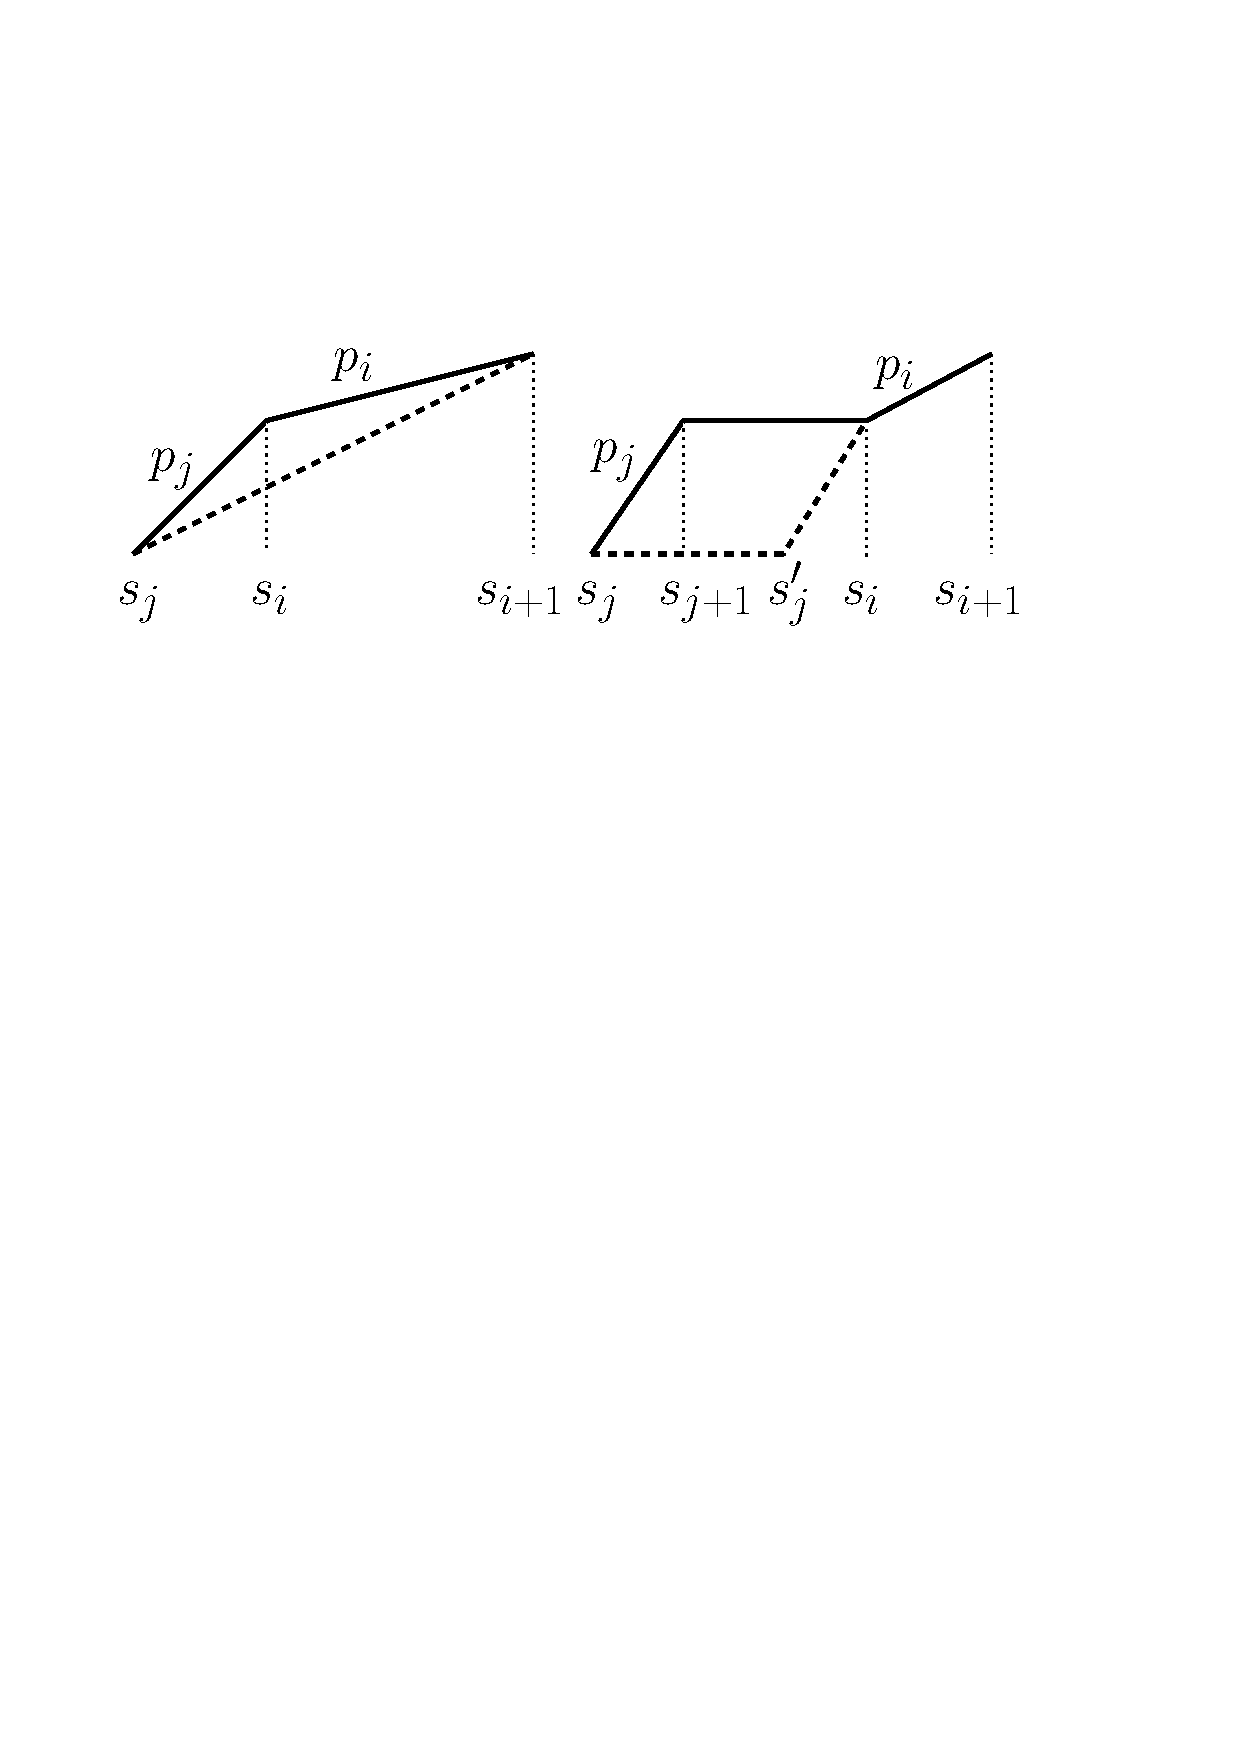
\includegraphics[width=8cm]{Lemma1.pdf}}
\caption{Figure showing the two cases of Lemma \ref{lemma_increasing_power}, \textit{Case 1} (left)  and \textit{Case2} (right) with $p_i>p_j$.}\label{Lemma1}
\end{figure}

\begin{lemma}
The optimal solution to Problem 1 may not be unique, but there always exists an optimal solution where once transmission has started, the receiver remains '\textit{on}' until the transmission is complete. \label{lemma_nobreaks}
\end{lemma}
\begin{proof}
The proof involves showing that we can generate an optimal solution with no breaks in transmission from any other optimal solution. Let the optimal policy be $\{\textbf{p},\textbf{s},N\}$. Now, if $p_i\neq 0,\forall \ i$, then we are done. Suppose some of $p_i$'s, say $p_{i_1},p_{i_2},...,p_{i_k}=0$ for some $k<N$, where $i_1<i_2<..<i_k$. Let $p_j$ be the first non-zero power after $p_{i_1}$. Consider a new policy which is same as policy $\{\textbf{p},\textbf{s},N\}$ till time $s_{i_1-1}$ and after time $s_{j}$. But, it keeps the receiver \textit{off} for a period of $(s_{j}-s_{i_1})$ starting from time $s_{i_1-1}$ and transmit with power $p_{i_1-1}$ from time $s_j'=(s_{i_1-1}+s_{j}-s_{i_1})$ till $s_j$. This policy transmits same amount of bits in same time as policy $\{\textbf{p},\textbf{s},N\}$ and also satisfies all constraints. So this policy is also optimal. But, in this policy the receiver \textit{off} duration, $(s_{j}-s_{i_1})$, has been shifted to left as shown in Fig.\ref{fig_Lemma2} (a). We continue this process of shifting the receiver \textit{off} period to left again and again to generate new optimal  policies till we reach a policy where the receiver is \textit{off} for time $(s_{j}-s_{i_1})$ from $s_1$ as shown in Fig. \ref{fig_Lemma2} (b). The start time of this policy (the one showed with solid line in Fig. \ref{fig_Lemma2} (b)) can now be changed to $s_1'=(s_1+s_{j}-s_{i_1})$. 

Similarly, we shift the receiver \textit{off} period corresponding to $p_{i_2},...,p_{i_k}$ till the total \textit{off} period is shifted to the beginning of transmission. This will result in a policy which starts after time $s_1$ and ends at time $s_{N+1}$, but the transmission power never goes zero in-between. Such a policy is also optimal and has no breaks.
\end{proof}
\begin{figure}[htb]
  \centering
  \centerline{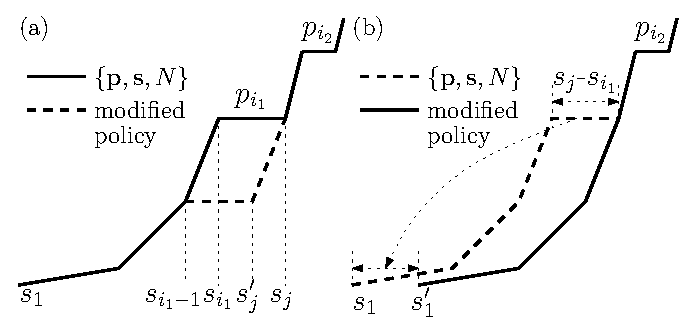
\includegraphics[width=8cm]{Lemma2.eps}}
\caption{Illustration of Lemma \ref{lemma_nobreaks}. Receiver \textit{off} time of $s_{j}-s_{i_1}$ is progressively shifted to left as shown in (a) to (b).}\label{fig_Lemma2}
\end{figure}
In rest of the paper, whenever we refer to the optimal solution for Problem 1, we assume it is the one with no breaks in transmission.
%This is equivalent to saying that there are no breaks during transmission in an optimal solution. Again, we shall prove this by contradiction. In the optimal solution, suppose the receiver is \textit{off} for some period after transmission starts. Let the transmission power before the break is $p_1$ and after the break is $p_2$. Considering Lemma \ref{lemma_increasing_power}, $p_1<p_2$, as shown in Fig. \ref{Lemma2_figure} (a). Consider the policy where we keep the receiver \textit{off} from time $A$ to $B'=(A+C-B)$. Now, an energy arrival can occur at the transmitter at any time between $A$ to $D$. If there is no energy arrival then transmitting at a constant rate from $B'$ to $D$ would transmit more bits.
%
%$Case 1:$ If the energy arrival is between $A$ and $B'$, then it can be easily seen that transmitting at a constant rate from $B'$ to $D$ would be better due to concavity of $g(p)$.
%
%$Case 2:$ If the arrival is between $B'$ and $C$ (say $C'$), then again transmitting at a same rate $p_1$ from $B'$ to $C'$ and  at a constant rate from $C'$ to $D$ would deliver more number of bits. In the worst case, an energy arrival occurring at $C$ would make this scenario transmit equal number of bits as the original scenario.
%
%$Case 3:$ If there is an energy arrival from $C$ to $D$ (say $D'$), then transmitting at maximum possible constant power form $B'$ to $D'$ and then at same rate $p_2$ from $D'$ to $D$ would deliver more bits to the receiver.
%
%Applying the above scenarios iteratively we could shift the receiver \textit{off} duration $(C-B)$ to the beginning of transmission and still, at worst case, transmit equal number of bits in same total time. Hence having a break in between transmission is always discouraged. This also gives us an idea of why the optimal solution may not be unique.
%\end{proof}
%
%\begin{figure}[htb]
%\centering
%\centerline{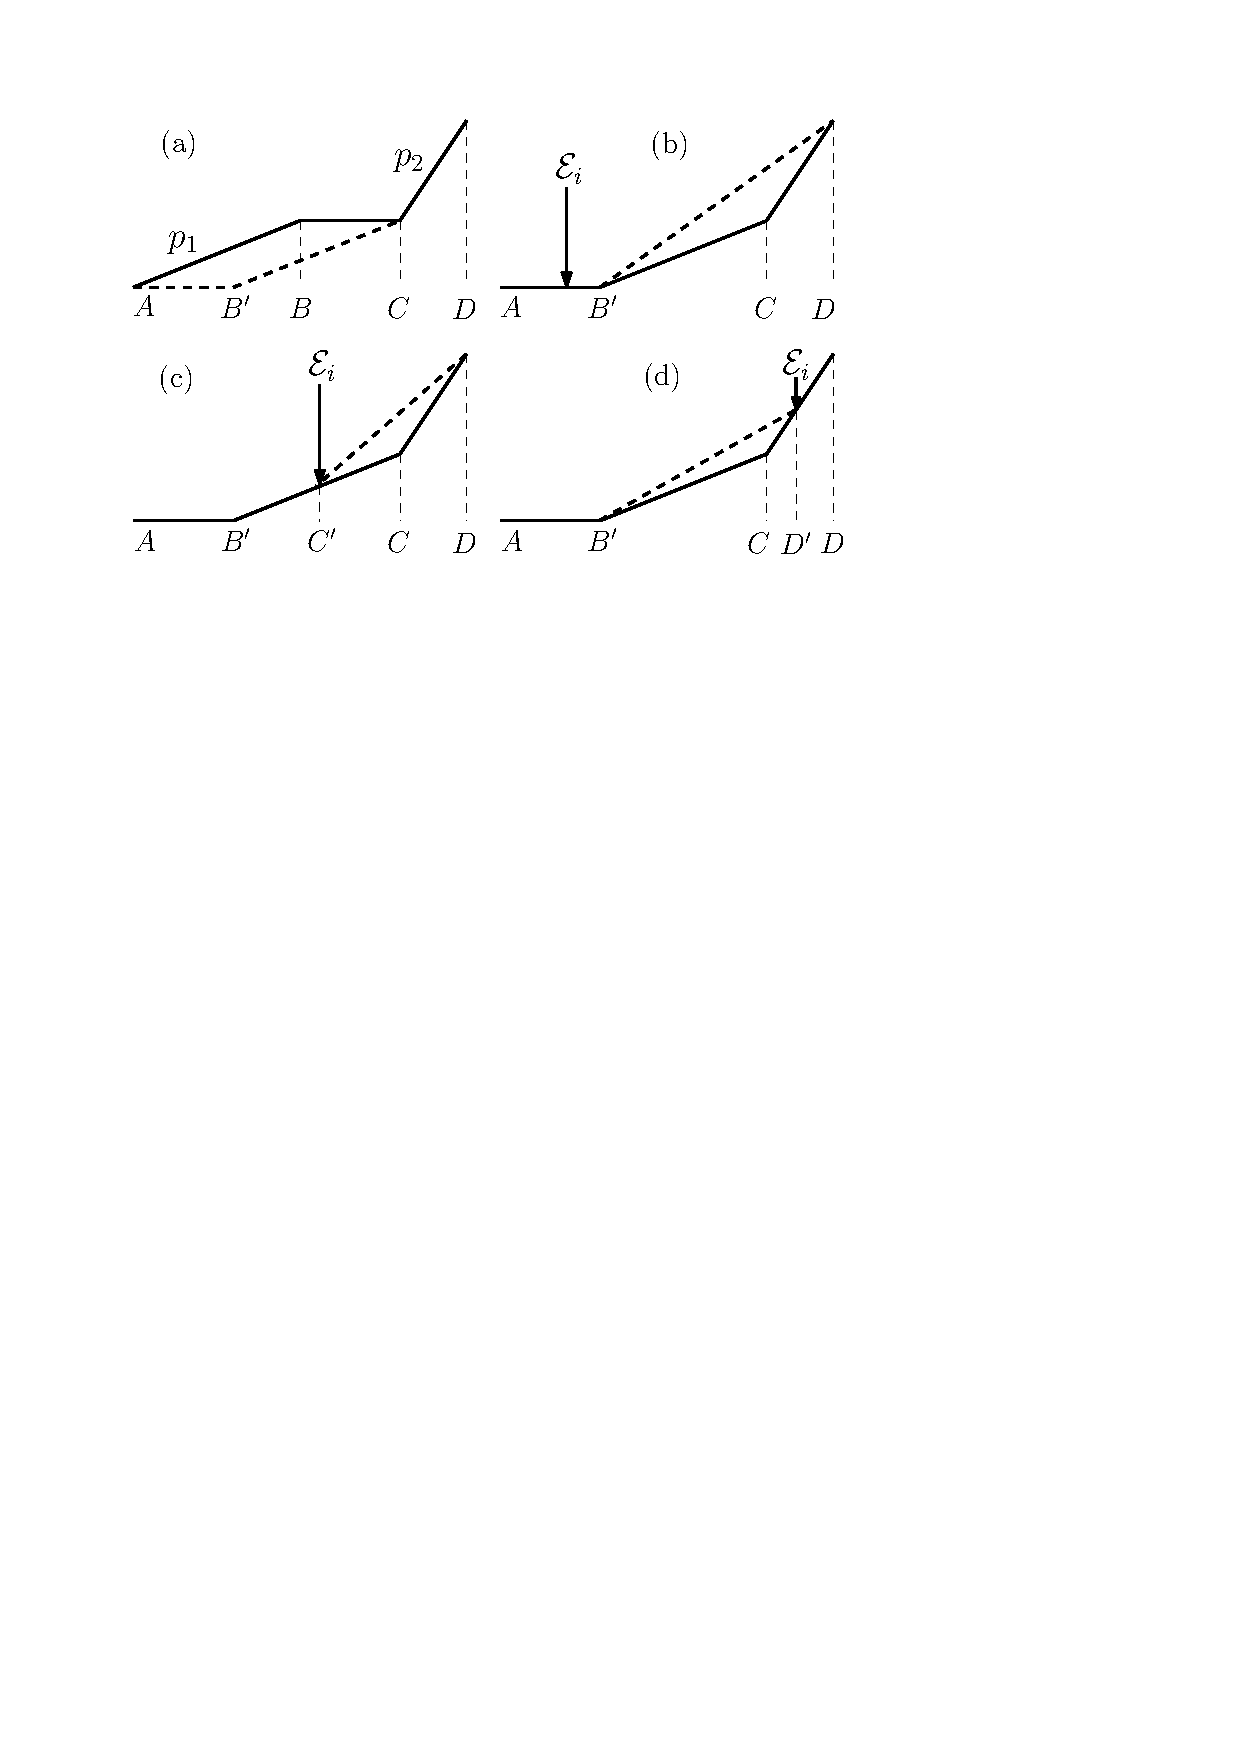
\includegraphics[width=8cm]{Lemma2.pdf}}
%\caption{Figure showing the three cases of Lemma \ref{lemma_nobreaks}, (a) the original scenario, (b) \textit{Case 1}, (c) \textit{Case 2} and (d) \textit{Case3} with $p_1>p_2$.}
%\label{Lemma2_figure}
%\end{figure}

\begin{lemma}
In an optimal solution with no breaks, the transmission power can only change at the time instants when energy arrives at the transmitter. The total energy used for transmission till that instant equals the total energy harvested upto that instant. The time instant where the transmission policy ends also satisfies this property.
\label{lemma_energy_consumed} 
\end{lemma}
\begin{proof}
Keeping in mind Lemma \ref{lemma_increasing_power} and \ref{lemma_nobreaks}, in the optimal solution $\{\textbf{p}, \textbf{s}, N\}$, transmission starts at $s_1$ and ends at $s_{N+1}$ without stopping in-between. Further, the transmission powers are also increasing. Assuming such a structure, the proof of this Lemma can be argued in similar terms of Lemma 2,3 in \cite{Yang}. 
\end{proof}	

\begin{lemma}
Consider two policies $\{\textbf{p},\textbf{s},N\}$  and $\{\bm{\widetilde{p}},\bm{\widetilde{s}},N\}$ ,which are feasible with respect to energy constraint \eqref{pb1_constraint_bits}, have non-decreasing powers and transmit same number of bits in total. If $\widetilde{p}_1=p_1-\alpha,\widetilde{p}_2=p_2,..,\widetilde{p}_{N-1}=p_{N-1},\widetilde{p}_N=p_N+\beta $ and $\widetilde{s}_1=s_1-\gamma,\widetilde{s}_2=s_2,..,\widetilde{s}_{N-1}=s_{N-1},\widetilde{s}_N=s_N+\delta $, where $\gamma=\dfrac{\alpha}{p_1-\alpha}(s_2-s_1)$, $\delta =\dfrac{\beta}{p_N+\beta}(s_{N+1}-s_N)$ and $\alpha ,\beta$ are positive constants, then 
\begin{equation}
(\widetilde{s}_{N+1}-\widetilde{s}_1)>(s_{N+1}-s_1).
\end{equation}
\label{lemma_increase_time}
\end{lemma}
\begin{proof}
The two policies $\{\textbf{p},\textbf{s},N\}$  and $\{\bm{\widetilde{p}},\bm{\widetilde{s}},N\}$ are shown in Fig. \ref{lemma4}. For every $\beta$ we can find a value of $\alpha$ such that the number of bits transmitted in policy $\{\bm{\widetilde{p}},\bm{\widetilde{s}},N\}$ remains the same as policy $\{\textbf{p},\textbf{s},N\}$. So, excluding the common parts in the transmission policy $\{\textbf{p},\textbf{s},N\}$ and $\{\bm{\widetilde{p}},\bm{\widetilde{s}},N\}$, we can equate
\begin{align}
&g(p_N)(s_{N+1}-s_N)+g(p_1)(s_2-s_1)\nonumber
\\
&=g(\widetilde{p}_N)(\widetilde{s}_{N+1}-\widetilde{s}_N)+g(\widetilde{p}_1)(\widetilde{s}_2-\widetilde{s}_1)\nonumber,
\\
&\implies (p_N+\beta)p_N\frac{\delta}{\beta}\left(\frac{g(p_N)}{p_N}-\frac{g(p_N+\beta)}{p_N+\beta}\right)\nonumber
\\
&=(p_1-\alpha)p_1\frac{\gamma}{\alpha}\left(\frac{g(p_1-\alpha)}{p_1-\alpha}-\frac{g(p_1)}{p_1}\right).\label{bits_equal}
\end{align}
$\exists$ $p_N':p_N<p_N'<p_{N}+\beta$ and $p_1':p_1-\alpha<p_1'<p_{1}$ such that
\begin{align}
&\frac{d}{dp} \frac{g(p)}{p} \bigg{\vert}_{p=p_N'}=\frac{1}{\beta}\left(\frac{g(p_N+\beta)}{p_N+\beta}-\frac{g(p_N)}{p_N}\right),\label{diff_1}
\\
&\frac{d}{dp} \frac{g(p)}{p}\bigg{\vert}_{p=p_1'}=-\frac{1}{\alpha}\left(\frac{g(p_1-\alpha)}{p_1-\alpha}-\frac{g(p_1)}{p_1}\right)\label{diff_2}.
\end{align}
Substituting (\ref{diff_1}) and (\ref{diff_2}) into (\ref{bits_equal}) we get,
\begin{align}
&\delta(p_N+\beta)p_N\frac{d}{dp} \frac{g(p)}{p}  \bigg{\vert}_{p=p_N'}
=\gamma(p_1-\alpha)p_1\frac{d}{dp} \frac{g(p)}{p} \bigg{\vert}_{p=p_1'}.\label{bits_equal1}
\end{align}
It can be verified that $\dfrac{d}{dp} \dfrac{g(p)}{p}$ is a decreasing function of $p$ using \eqref{property_concave}. As $p_1'<p_N'$, equation (\ref{bits_equal1}) implies $\gamma >\delta$. Hence the time for which transmission occurs in the policy $\{\bm{\widetilde{p}},\bm{\widetilde{s}},N\}$, $\left( s_{N+1}-s_1+\gamma-\delta\right)$, is greater than transmission time in policy $\{\textbf{p},\textbf{s},N\}$ i.e. $(s_{N+1}-s_1)$.
\end{proof}
\begin{figure}
\centering
  \centerline{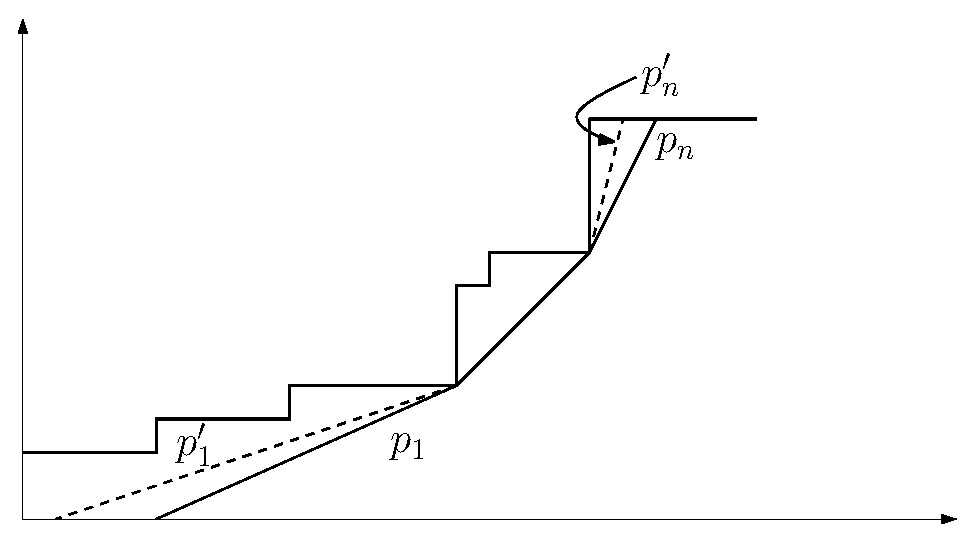
\includegraphics[width=8cm]{Lemma4.eps}}
\caption{Illustration of the proof of Lemma \ref{lemma_increase_time}.}\label{lemma4}
\end{figure}

\begin{lemma}
If the receiver has energy to stay \textit{'on'} for $\TRx_0$ time, then either the transmitter will transmit for the entire duration $\TRx_0$ or the transmitter will begin transmission at time $t=0$, in which case it stays \textit{on} for less than or equal to $\TRx_0$ time. 
\label{transmission_duration}
\end{lemma}
\begin{proof}
We will prove this by contradiction. Suppose the optimal transmission policy $\{\textbf{p},\textbf{s},N\}$ does not begin transmitting at time $t=0$ and transmits for a duration $(s_{N+1}-s_1)< \TRx_0$. Now, consider a policy $\{\bm{\widetilde{p}},\bm{\widetilde{s}},N\}$ as defined in Lemma \ref{lemma_increase_time}. By Lemma \ref{lemma_energy_consumed}, policy $\{\textbf{p},\textbf{s},N\}$ exhausts all energy at epochs $s_i$'s. So, $s_{2}$ is the first energy arrival which is on the boundary of energy constraint (\ref{pb1_constraint_energy}) i.e. $U(s_2)=\ETx(s_2^-)$ and $s_{N}$ is the last epoch satisfying $U(s_N)=\ETx(s_N^-)$. Hence we can choose $\alpha ,\beta$ such that policy $\{\bm{\widetilde{p}},\bm{\widetilde{s}},N\}$ would be feasible with respect energy constraint (\ref{pb1_constraint_energy}). By Lemma \ref{lemma_increase_time}, the time for which transmission occurs in the policy $\{\bm{\widetilde{p}},\bm{\widetilde{s}},N\}$, $\left( \widetilde{s}_{N+1}-\widetilde{s}_1\right)$, is greater than transmission time in policy $\{\textbf{p},\textbf{s},N\}$ i.e. $(s_{N+1}-s_1)$. As $s_{N+1}-s_1<\TRx_0$, we can further reduce $\alpha,\beta$ to arbitrarily small positive values so that $(s_{N+1}-s_1)<\left( \widetilde{s}_{N+1}-\widetilde{s}_1\right)<\TRx_0$ holds. With this choice of $\alpha,\beta$, policy $\{\bm{\widetilde{p}},\bm{\widetilde{s}},N\}$ is feasible with constraints  (\ref{pb1_constraint_bits}), (\ref{pb1_constraint_energy}), (\ref{pb1_constraint_time}) and contradicts the optimality of policy $\{\textbf{p},\textbf{s},N\}$ (as $\{\bm{\widetilde{p}},\bm{\widetilde{s}},N\}$ finishes before the optimal policy). This concludes that $s_{N+1}-s_1=\TRx_0$ (if $s_1\neq 0$) in optimal policy.
\end{proof}
% !TEX root = OptimalOffline.tex

\begin{figure}
\label{lemma4}
\centering
  \centerline{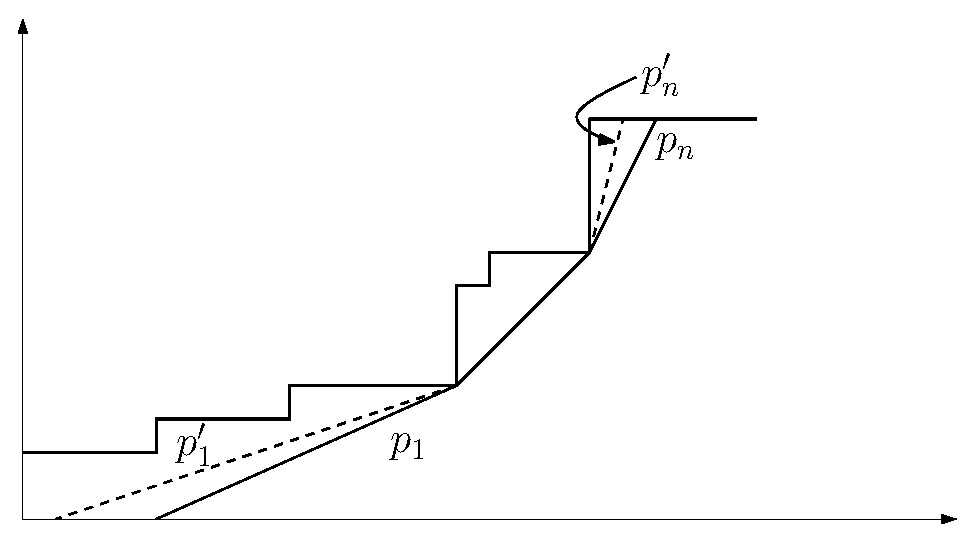
\includegraphics[width=8cm,height=50mm]{Lemma4.eps}}
\caption{Illustration of the proof of lemma \ref{transmission_duration}. The dotted line represents the policy where the first power of transmission is slightly reduced, to make the transmissino finish earlier}
\end{figure}

\begin{lemma}
If the receiver has enough energy to stay on for $T$ time, then either the transmitter will transmit for the entire duration $T$ or the transmitter will begin transmission at time $t=0$.
\label{transmission_duration}
\end{lemma}
\begin{proof}
We will prove this by contradiction. Suppose the optimal transmission policy $\{\textbf{p},\textbf{s},N\}$ does not begin transmitting at time $t=0$ and transmits for a duration $s_{N+1}-s_1 < T$.

If we reduce $p_1$ slightly to $p_1-\delta p_1$, we will have transmitted more bits by time $s_N$. Therefore at the end we can transmit with a power $p'_N > p_N$ and complete our transmission at an earlier time.

Thus we can keep lowering our first transmission power until we either exhaust our transmission duration $T$ or we hit the origin.
\end{proof}

Concluding the results of all Lemmas our optimal policy $\{\textbf{p},\textbf{s},N\}$ must have change transmission powers at energy arrival epochs only i.e. $\forall i,\ s_i=t_j$ for some $j$. At these epochs we exhaust the total energy available with us i.e. $U(s_i^-)=\ETx(s_i^-)$. The transmission powers are also non decreasing with time and we exhaust the total 'receiver time' time given to us, if we do not start transmitting from origin.

Now that we have gained some knowledge of the structure our algorithm has to follow, we consider an example to approach Problem 1. 

Suppose we are given that the receiver can be \textit{on} for a maximum duration of $T$. Our goal is to find a transmission policy so that we can minimize the time at which the transmission is completed. To do this, we shall first find a feasible solution i.e. one which satisfies all constraints (\ref{pb1_constraint_bits})-(\ref{pb1_constraint_time}) and keep improving upon it, until we have a solution that follows all our Lemma 1-4 and hits the boundary on some or all of the constraints (\ref{pb1_constraint_bits})-(\ref{pb1_constraint_time}). 

We need an initial feasible solution to begin with. For this, we find the minimum energy required by the transmitter so that the transmission can be completed in duration $T$ with a constant power. That is, the first $n$ such that
\begin{equation}
T g\left(\frac{\ETx(t_n)}{T}\right)\geq B_0.
\end{equation}
Let $\widetilde{T}$ be the time duration such that
\begin{equation}
\widetilde{T}g\left(\frac{\ETx(t_n)}{\widetilde{T}}\right)=B_0.
\end{equation}
Let $\tilde{p}=\frac{\ETx(t_n)}{\widetilde{T}}$. We try to transmit with this power starting at t=0. If it does not violate the energy constraint (\ref{pb1_constraint_energy}), we are done with the optimal solution and our transmission is completed in $\widetilde{T}$ time.

If not, we start the transmission as early as possible, such that the transmission is feasible with respect to (\ref{pb1_constraint_energy}). This transmission policy, will encounter atleast one epoch where total energy consumed till that epoch is equal to the total energy harvested upto it. Let time $Q$ be the first point where this happens. This is shown in Figure \ref{straight}. Till now we have not argued why we chose such a policy to start with. In fact the next Lemma shows that this starting solution is a 'good' estimate as both the optimal policy and the above policy run out of all their energy at epoch $Q$.

\begin{figure}
\label{straight}
\centering
  \centerline{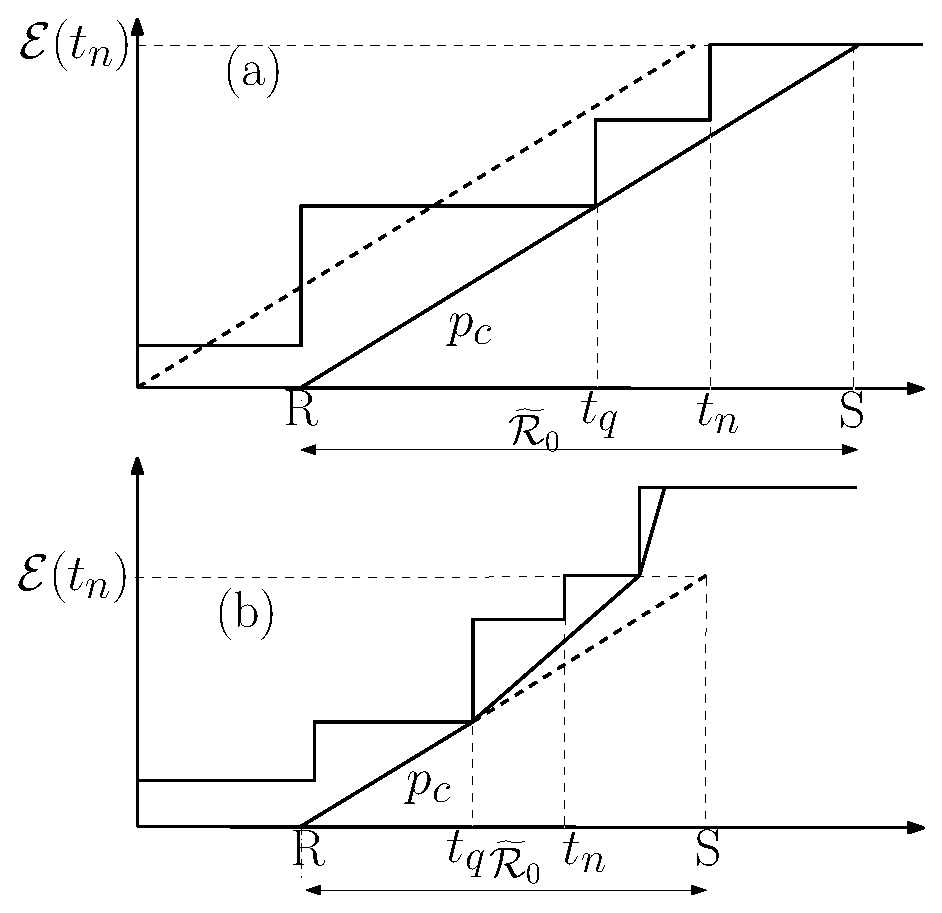
\includegraphics[width=8cm,height=4cm]{straight.eps}}
\caption{Figure showing point Q.}
\end{figure}

\begin{lemma}
In every optimal solution, at energy arrival epoch $Q$, $U(Q^-)=\ETx(Q^-)$.
\label{lemma_Q}
\end{lemma}
\begin{proof}
We shall prove this by contradiction. Let the start and end times of the constant power transmission policy described above be $R$ and $S$ receptively. We make the following claims:

\textbf{Claim 1:} Every optimal transmission policy begins transmission at or before time $R$

Since, $S-T=\widetilde{T}\le T$ (by Lemma \ref{transmission_duration}) if a transmission policy has to finish before $S$, it has to start before time $\max(S-T,0) \le \max(R,0)$. 

%Since we are transmitting all the bits at the maximum possible power, no policy that starts after $R$ can finish before $S$. Therefore, any policy that starts after $R$ cannot be optimal.

\textbf{Claim 2:} Every optimal transmission policy ends transmission at or before time $S$.
This follows immediately from the fact that the policy is optimal.

Let $Q$ equal to time $t_i$ for some $i\in\mathbb{N}$. Suppose we have an optimal transmission policy that does not exhaust all its energy at time $Q$ i.e. $U(t_j)<\ETx(t_i^-)$. By Lemma \ref{lemma_energy_consumed} it does not change its transmission power at $t_i$. Let the transmission power of optimal policy be $p$ at $t_i$. This does not change till an epoch, say $t_j$. Now, $t_j<S$ by \textit{Claim 2}. Further the constant power policy exhausts all its energy by $Q$. So,
\begin{align}
&\tilde{p}(t_i-R)=\ETx(t_i^-)\label{eqlemmaQ1}.
\end{align}
But, by constraint (\ref{pb1_constraint_energy})
\begin{align}
&\tilde{p}(t_i-R)+\tilde{p}(t_j-t_i)\le \ETx(t_j^-),
\\
&\implies \tilde{p}(t_j-t_i)\stackrel{(\ref{eqlemmaQ1})}{\le} \ETx(t_j^-)-\ETx(t_i^-),\\
&\implies \tilde{p}(t_j-t_i)< \ETx(t_j^-)-U(t_i)=p(t_j-t_i),\\
&\implies \tilde{p}<p .\label{eqlemmaQ2}
\end{align}
If the optimal policy does have a power higher than $\tilde{p}$ at $t_i$, then it must have the same power of transmission either from some epoch, say $t_k$, or from the beginning of transmission. If $t_k>R$, we can show that the constant power policy is infeasible with respect to constraint (\ref{pb1_constraint_energy}) at $t_k$. If $t_k<R$ it becomes infeasible at time $R$. If the optimal policy starts transmission with power $p$, it has to begin transmission after time $R$ which follows from equation (\ref{eqlemmaQ2}). This violates \textit{Claim 1}. Therefore every optimal transmission policy must use all energy till epoch $Q$.
\end{proof}

Now that we have a starting point, we shall proceed to improve upon this policy as follows. Let $t_{lt}$ and $t_{rt}$ be the first and last energy arrival epochs where the power of transmission changes. 
As it is evident, initially both $t_{lt}$ and $t_{rt}$ are set to point $Q$. Now, will iteratively try to omporove on the transmission curve to the left and the right of point $Q$ respectively. 
Keeping in mind Lemma \ref{transmission_duration}, we solve 
\begin{align}
xg\left(\frac{\ETx(t_{lt})}{x}\right) + (T-x)g\left(\frac{\ETx(n)-\ETx(t_{rt})}{T-x}\right) = B
\end{align}
Notice that $t_{lt} - x$ and $t_{rt} + T-x$ will give us the start and end points of this iteration. Now, we transmit at power $p_{lt} = \frac{\ETx(t_{lt})}{x}$ prior to $t_{lt}$ and $p_{rt} = \frac{\ETx(n) - \ETx(t_{rt})}{T-x}$ after $t_{rt}$. 
If this policy is feasible, then we check for the following. First, we make sure that at the end point, all the available energy is used up, because of it isn't, we can transmit at a higher power and finish earlier. 
If all the energy is not used up, we repeat our iteration, setting $n$ to $k$, where $t_k$ is the last energy arrival epoch before our end point, $t_{rt} + T-x$  \\
If all the energy is used up, then we set $t_{rt}$ to the end point. 
Also, we make sure that our start point, is not before the origin. If the start point is negative, we set it to origin. Now if our start point happend to hit origin at any point in the algorithm, then our problem can be 
solved using the algorithm described by Yang et al in \cite{Yang}. So, should our start point hit origin, we simply use their algorithm for the allocations beyond $t_{rt}$.

If the policy is unfeasible on the right, we select the corner point $t_i$ with the minimum slope from $t_{rt}$ and transmit with power $\frac{\ETx(t_i) - \ETx(t_{rt})}{t_i-t_{rt}}$ between the two points and set $t'_{rt} = t_{rt}$ and $t_{rt} = t_i$ and repeat the process.\\
If the policy is unfeasible on the left, we follow a similar process, be selecting the corner point $t_j$ with the \textit{maximum} slope from point $t_{rt}$.\\
At the end of every iteration we reset our $T$ to $ T - (t_{rt} - t'_{rt}) - (t'_{lt} - t_{lt})$ and we subtract the number of bits transferred between $t_{lt}$ and $t_{rt}$ from $B$



\begin{table}
\begin{minipage}[b]{8cm}
\caption{Offline Algrithm for finding optimal transmission policy, given transmission duration}
\begin{tabular}{p{7cm}}
\hline \textbf{Input}: Bits to transmit $B_0$, transmission duration $T_0$.\\
\hline
\\
\textbf{Initialize:}$B = B_0$, $T = \TRx_0$, DEQUE $S$, hitorig = $0$
\\
% \textbf{While} $Tg(\ETx(n)) < B$
% \\
% \hspace{4mm} $n = n+1$
$n=\displaystyle \argmin_k\left(\left\{t_k | Tg\left(\frac{\ETx(t_k)}{T}\right)\geq B\right\}\right)$
\\
Solve for $\widetilde{T}: \widetilde{T}g\left(\dfrac{\ETx(t_n)}{\widetilde{T}}\right) = B$
\\
$p_0=\dfrac{\ETx(n)}{\widetilde{T}}$
\\
% \textbf{for} $i=0,1,2,...n$ \textbf{do}
% \\
% \hspace{4mm}flag=1
% \\
% \hspace{4mm}\textbf{for} $j=i,i+1,i+2,...,n$ \textbf{do}
% \\
% \hspace{7mm}\textbf{if} $p_0t_j + (\ETx(t_i) - p_0t_i) > \ETx(t_j)$
% \\
% \hspace{10mm}$flag=0$
% \\
% \hspace{10mm}break
% \\
% \hspace{7mm}\textbf{end if}
% \\
% \hspace{4mm}\textbf{end for}
% \\
$q=\displaystyle \argmin_k\left(\left\{ t_k | (\ETx(t_k) - p_0t_k) + p_0t_j \leq \ETx(t_j) \forall j\in[0,n] \right\}\right)$
\\
% \hspace{4mm}\textbf{if} $flag=1$
% \\
% \hspace{7mm}$t_{lt} = t_{rt} = t_i$
% \\
% \hspace{7mm} $S$.append($t_i$)
% \\
% \hspace{7mm}break
% \\
% \hspace{4mm}\textbf{end if}
% \\
% \textbf{end for}
% \\
%$n = \displaystyle \argmax_{k\in\mathbb{N}}\left(\left\{t_k | t_k<\dfrac{E_n - \ETx(t_i) - p_0t_i}{p_0}\right\}\right)$
$t_{lt} = t_{rt} = t_q$
\\
$S$.append($t_q$)
\\
\textbf{while} $B>0$
\\
\hspace{4mm}\textbf{Solve}: $xg\left(\dfrac{\ETx(t_{lt})}{x}\right)+(T-x)g\left(\dfrac{\ETx(t_n)-\ETx(t_{rt})}{T-x}\right) = B_0$
\\
\hspace{4mm}$p_{lt} = \dfrac{\ETx(t_{lt})}{x}$
\\
\hspace{4mm}$p_{rt} = \dfrac{\ETx(t_n)-\ETx(t_{rt})}{T-x}$
\\
\hspace{4mm}$t_{start} = t_{lt} - \dfrac{\ETx(t_{lt})}{p_{lt}}$
\\
\hspace{4mm}$T_{lt} = \{t_i | t_i >t_{start}, t_i < t_{lt}   \}$
\\
\hspace{4mm}$t=0$
\\
\hspace{4mm}\textbf{For} $t_i \in T_{lt}$
\\
\hspace{7mm}\textbf{If} $p_{lt}t_i + (\ETx(t_{lt}) - p_{lt}t_{lt}) > \ETx(t_{i-1})$
\\
\hspace{10mm}$t'_{lt} = t_{lt}$
\\
\hspace{10mm}$t_{lt} = \displaystyle \argmax_{j\in(T_{lt})}\left(\dfrac{\ETx(t_{lt}) - \ETx(j)}{t_{lt}-j}\right)$
\\
\hspace{10mm}$S$.prepend($t_{lt}$)
\\
\hspace{10mm}$t_{start} = t_{lt} - \dfrac{\ETx(t_{lt})}{p_{lt}}$
\\
\hspace{10mm}$t=1$
\\
\hspace{10mm}\textbf{break}
\\
% \hspace{7mm}\textbf{else}
% \\
% \hspace{10mm} $t_{lt} = max(t_{lt} - \dfrac{\ETx(t_lt)}{p_{lt}} , 0)$
% \\
\hspace{7mm}\textbf{end if}
\\
\hspace{4mm}\textbf{End For}
\\
\hspace{4mm}\textbf{if} $t=0$
\\
\hspace{7mm}$t_{lt} = max\left(t_{start} , 0\right)$
\\
\hspace{7mm}\textbf{if} $t_{lt} = 0$ 
\\
\hspace{10mm}hitorig = 1
\\
\hspace{10mm}\textbf{break}
\\
\hspace{4mm}\textbf{end if}
\\
\hspace{4mm}$T_{rt} = \{t_k|t_k>t_{rt}, t_k<t_{rt}+p_{rt}\}$
\\
\hspace{4mm}$u=0$
\\
\hspace{4mm}\textbf{For} $t_i \in T_{rt}$
\\
\hspace{7mm}\textbf{If} $p_{rt}t_i + (\ETx(t_{rt}) - p_{rt}t_{rt}) > \ETx(t_i)$
\\
\hspace{10mm}$t'_{rt} = t_{rt}$
\\
\hspace{10mm}$t_{rt} = \displaystyle \argmin_{j\in(S_{rt})}\left(\dfrac{\ETx(t_j)-\ETx(t_{lrt})}{t_j-t_{rt}}\right)$
\\
\hspace{10mm}$S$.append($t_{rt}$)
\\
\hspace{10mm}$t_{stop} = t_{rt} + \frac{\ETx(E_n)}{p_{rt}}$
\\
\hspace{10mm}$u=1$
\\
\hspace{10mm}\textbf{break}
\\
% \hspace{7mm}\textbf{else}
% \\
% \hspace{10mm} $t_{rt} = t_{rt} + \dfrac{\ETx(t_n)-\ETx(t_rt)}{p_{rt}}$
% \\
% \hspace{10mm}\textbf{If} $t_{rt}>t_{n}$
% \\
% \hspace{13mm}\textbf{While} $t_n < t_{rt}$
% \\
% \hspace{16mm} $n=n+1$
% \\
% \hspace{13mm} \textbf{end while}
% \\
% \hspace{13mm} $t_{rt} = t'_{rt}$
% \\
% \hspace{10mm}\textbf{end for}
% \\
\hspace{7mm}\textbf{end if}
\\
\hspace{4mm}\textbf{End For}
\\
% \textbf{Write the following block in a better way}
% \\
\hspace{4mm}\textbf{if} ($u=0$ and $\ETx(t_{stop}) < \ETx(n) $ )
\\
\hspace{7mm} $n=\displaystyle \argmax_k\left(\left\{t_k | t_k< t_{stop} \right\}\right)$
\\
% \hspace{7mm} $t_{rt} = t_{rt} + \dfrac{\ETx(t_n)-\ETx(t_rt)}{p_{rt}}$
% \\
% \hspace{7mm}\textbf{If} $t_{rt}>t_{n}$
% \\
% \hspace{10mm}\textbf{While} $t_n < t_{rt}$
% \\
% \hspace{13mm} $n=n+1$
% \\
% \hspace{10mm} \textbf{end while}
% \\
% \hspace{7mm} $t_{rt} = t'_{rt}$
% \\
% \hspace{7mm}\textbf{end for}
% \\
\\
\hspace{4mm}\textbf{else if}($u=0$)
\\
\hspace{7mm}$t_{rt} = t_{stop}$
\\
\hspace{7mm}$t_{lt} = t_{start}$
\\
\hspace{4mm}\textbf{end if}
\\
\hspace{4mm} $T = T - (t_{rt}-t'_{lt}) - (t'_{lt} - t_{lt})$
\\
\hspace{4mm}$B = B -  (t'_{lt}-t_{lt})g(\dfrac{\ETx(t'_{lt})-\ETx(t_{lt})}{t'_{lt}-t_{lt}}) - (t_{rt}-t'_{rt})g(\dfrac{\ETx(t_{rt})-\ETx(t'_{rt})}{t_{rt}-t'_{rt}})$
\\
\textbf{end while}
\\
\textbf{if} hitorig = 1
\\
\hspace{4mm}
Apply previous algorithm after $t_{rt}$
\\
\textbf{end if}
\end{tabular}
\end{minipage}
\end{table}

%!TEX root = OptimalOffline.tex
%input{Siddhartha}
\begin{theorem}
Let a transmission policy to solve Problem 1 is given by power vector $\textbf{p}=[p_1,p_2,..,p_N]$ and the start time of transmission for the corresponding power be given by vector $\textbf{s}=[s_1,s_2,..,s_N]$, for some $N\in \mathbb{N}$. The transmission ends at time $s_{N+1}$. Now such a policy is optimal if and only if it satisfies the following structure.
\label{th_algo1_1}
\begin{align}
&\sum_{i=1}^{i=N}g(p_i)(s_{i+1}-s_i)=B_0\label{claim1}
\\
&\nonumber s_{N+1}-s_1=T^R_0 				&&\text{ , if } s_1>0
\\
& \text{ or } s_{N+1}\le T^R_0 				&&\text{ , if } s_1=0\label{claim2}
\\
&\nonumber s_{n+1}=\argmin_{t_i: s_n < t_i \le s_{N+1}} CP(t_i,s_n)
\\
&\text{ and } p_n=CP(s_{n+1},s_n)\label{claim3}
\\
&\exists s_j:s_j\in \textbf{s} \text{ and } s_j=Q\label{claim4}
\end{align}
for $n=\{ 1,2,..,N-1\}$.
\end{theorem}
\begin{proof}
First we show that the optimal policy should have the given structure. The proof follows the method of  contradiction. We establish structure (\ref{claim3}) at first. Assume an optimal policy that satisfies Lemmas 1 to 6 and does not satisfy the given structure (\ref{claim3}). Specifically, say the policy be same as structure (\ref{claim3}) from time $s_{1}$ to $s_n$, for some $n\in \{1,2,..,N\}$ but transmission power right after $s_n$ is not the minimum feasible constant power, i.e.
\begin{align}
p_n>CP(s',s_n)\text{ where } s'=\argmin_{t_i: s_n < t_i \le s_{N+1}} CP(t_i,s_n)\label{claim3_1}
\end{align}

\textit{Case1: }if $s'>s_{n+1}$ for some $n\in \{1,2,..,N-1\}$, then the energy that is used for transmission from time $s'$ to $s_{n+1}$ is given by $\ETx(s'-)-\ETx(s_{n+1}^-)$ in terms of Lemma 3. We claim that that there must be a time duration from $s'$ to $s_{n+1}$ for which the transmission power is less than $p_n$. If this claim is true then we violate lemma \ref{increasing_power} and hence contradict the assumption. Coming to the claim, if it does not hold i.e. transmission power at all points of time between $s_{n+1}$ to $s'$ is more than $p_n$, then the total energy used during this period can be lower bounded by $p_n(s'-s_{n+1})$. Next, we show that this energy is more that what is harvested during $s_{n+1}$ to $s'$ making it infeasible. As transmitting with $CP(s',s_n)$ power is a feasible between time $s'$ and $s_n$, $CP(s',s_n)(s_{n+1}-s_n)\le \ETx(s_{n+1}^-)-\ETx(s_{n}^-)$. So, 
\begin{align}
&\ETx(s'-)-\ETx(s_{n+1}^-) \le \ETx(s'-)-\ETx(s_{n+1}^-)
\\
&+(\ETx(s_{n+1}^-)-\ETx(s_{n}^-)-CP(s',s_n)(s_{n+1}-s_n))
\\
&=CP(s',s_n)(s'-s_{n+1})\stackrel{(\ref{claim3_1})}{<}p_n (s'-s_{n+1}).
\end{align}

\textit{Case2: }if $s'<s_{n+1}$, the transmission policy uses $p_n(s'-s_{n})$ energy from time $s_n$ to $s'$. But $\ETx(s'-)-\ETx(s_{n}^-)=CP(s',s_n)(s'-s_{n})\stackrel{\ref{claim3_1}}{<}p_n(s'-s_{n})$. So, energy used $p_n(s'-s_{n})$ is more than what is harvested making this case infeasible.

%Note that equation (\ref{claim1}) must be followed by the optimal policy as it is a constraint to the optimization problem 1. We move on to prove structure (\ref{claim2}). If $s_1=0$ then $s_{N+1}$ has to be less than or equal to $T^R_0$ due to constraint 1. When $s_1>0$, assume that $s_{N+1}-s_1<T^R_0$. Let $A$ be the first energy arrival such that $E(A)=\ETx(A^-)$. Similarly, let $B$ be the last energy arrival at which $E(B)=\ETx(B^-)$. Now consider the policy where power vector is given by $\{p_1-\alpha,p_1,p_2,..,p_{N-1},p_N,p_N+\epsilon \}$ and the corresponding time vector be given by $\{s_1-\beta,A,s_2,..,s_{N},B\}$ with the transmission ending at time $s_{N+1}-\gamma$, where $\epsilon$ is a small positive constant, $\beta=\frac{\alpha}{p_1-\alpha}(A-s_1) $, $\gamma= \frac{\epsilon}{p_N+\epsilon}(s_{N+1}-B)$. This policy finishes before the previous policy and hence contradicts its optimality only if we are able to show that it is feasible. Such a policy would be feasible with respect to the energy constraint keeping in mind that transmission with power $p_N+\epsilon $ from time $A$ to $s_{N+1}-\gamma$ was previously never on the boundary of feasibility constraint 1 and similarly for power $p_1-\alpha $. Now we see its feasibility with constraint 2. For every $\epsilon \rightarrow 0^{+}$ we can find a value of $\alpha$ such that the number of bits transmitted in this new policy remains the same as the previous one i.e. $B_0$. So, excluding the common terms from equating the number of bits boils to
%\begin{align}
%&\nonumber g(p_N)(s_{N+1}-B)+g(p_1)(A-s_1)
%\\
%&\nonumber =g(p_1-\alpha)(A-s_1+\beta)+g(p_N+\epsilon)(s_{N+1}-B-\gamma)
%\\
%&\nonumber\implies (s_{N+1}-B)(g(p_N)-g(p_N+\epsilon)\frac{p_N}{p_N+\epsilon})
%\\
%&=(A-s_1)(g(p_1-\alpha)\frac{p_1}{p_1-\alpha}-g(p_1))\label{bits}
%\end{align} 
%Now the total time for which the transmission is \textit{on} is $s_{N+1}-s_1+\beta-\gamma$.


Note that equation (\ref{claim1}) must be followed by the optimal policy as it is a constraint to the optimization problem 1. We move on to prove structure (\ref{claim2}). If $s_1=0$ then $s_{N+1}$ has to be less than or equal to $T^R_0$ due to constraint 1. When $s_1>0$, assume that $s_{N+1}-s_1<T^R_0$. Let $A$ be the first energy arrival such that $E(A)=\ETx(A^-)$. Similarly, let $B$ be the last energy arrival at which $E(B)=\ETx(B^-)$. Now consider the policy where power vector is given by $\{p_1+dp_1,p_1,p_2,..,p_{N-1},p_N,p_N+dp_N \}$ and the corresponding time vector be given by $\{s_1+ds_1,A,s_2,..,s_{N},B\}$ with the transmission ending at time $s_{N+1}+ds_{N+1}$, where $dp_N>0$ and  $dp_1,ds_1, ds_{N+1}<0$ . This policy finishes before the previous policy and hence contradicts its optimality only if we are able to show that it is feasible. Such a policy would be feasible with respect to the energy constraint keeping in mind that transmission with power $p_N$ from time $A$ to $s_{N+1}$ was previously never on the boundary of feasibility constraint 1 and similarly for power $p_1$. Now we see its feasibility with respect to constraint 2. It can be seen that
\begin{align}
&p_1ds_1=(A-s_1)dp_1\text{ , }p_Nds_{N+1}=-(s_{N+1}-B)dp_N
\end{align}
The number of bits transmitted from time $s_1$ to $A$ is given by $B_1=g(p_1)(A-s_1)$ and similarly, from $B$ to $s_{N+1}$ be given by $B_N=g(p_N)(s_{N+1}-B)$ under the previous policy. Noting that the number of bits sent in the two policies remains same we get,
\begin{align}
&\nonumber dB_1+dB_2=0
\\
&\nonumber\implies g'(p_1)(A-s_1)dp_1-g(p_1)ds_1
\\
&\nonumber +g'(p_N)(s_{N+1}-B)dp_N+g(p_N)ds_{N+1}=0
\\
&\nonumber\implies \frac{-ds_1}{-ds_{N+1}}=\frac{(g'(p_N)p_N-g(p_N))}{(g'(p_1)p_1-g(p_1)}
\end{align}
We can verify that $g'(p)p-g(p)$ is an increasing function of $p$ for $p>0$ due to concavity of $g(p)$. Hence $(-ds_1)\ge (-ds_{N+1})$. The time for which transmission is on in this policy is $s_{N+1}-s_1+ds_{N+1}-ds_1\ge s_{N+1}-s_1$. As $s_{N+1}-s_1<T^R_0$, we can choose arbitrarily small negative value of $ds_{N+1}$ so that $s_{N+1}-s_1\le s_{N+1}-s_1+ds_{N+1}-ds_1<T^R_0$ holds. So the new policy finishes earlier than the previous policy contradicting the optimality. This concludes that $s_{N+1}-s_1=T^R_0$ (if $s_1\neq 0$) in optimal policy.

Next, we prove the sufficiency of the structure. Let the power vector $\textbf{p}$ and time vector $\textbf{s}$ follow the structure. We need to show that this policy is optimal. Assume that there exists another policy given by $\{\textbf{p'},\textbf{s'}\}$ which abides by the Lemma 1-5 and is optimal, but does not follow the structure. We argue next that such a policy is not feasible and hence contradict its optimality. 

\textit{Case1}: If $s_1'>s_1\ge 0$ then by Lemmma  $s_{N'+1}'>s_{N+1}$. So policy $\{\textbf{p'},\textbf{s'}\}$ cannot be optimal. 

\textit{Case2}: Suppose $s_1'=s_1$. Let $s_i'$ be the first epoch for which $p_i'\ne p_i$ for some $i \in \{1,2,..,N\}$. By (\ref{claim3}), $p_i'>p_i$. If $s_{N'+1}'>s_{i+1}$, then the amount of energy used by policy $\{ \textbf{p'},\textbf{s'}\}$ in interval $[s_{i},s_{i+1}]$ is more than policy $\{\textbf{p},\textbf{s}\}$. But by Lemma, $\{\textbf{p},\textbf{s}\}$ uses all energy available by $s_{i+1}$. So policy $\{\textbf{p'},\textbf{s'}\}$ is not feasible with respect to the energy constraint. If $s_{N'+1}'\le s_{i+1}$, then it can be easily verified by property P4 that policy $\{\textbf{p'},\textbf{s'}\}$ transmits strictly less number of bits in interval $[s_i,s_{N'+1}]$ than the other policy in interval $[s_{i},s_{i+1}]$. Both policies being same till $s_i$, we conclude that policy $\{\textbf{p'},\textbf{s'}\}$ transmits less than $B_0$  bits and therefore it is not optimal.

\textit{Case3}: This case argues the infeasibility when $s_1'<s_1$. Unlike other cases this case is more rigorous. The idea of the proof is to show that if we start our transmission early and finish earlier than policy $\{\textbf{p},\textbf{s}\}$, we always take more transmission time which is going to violate the time constraint. First, we establish that the policy $\{\textbf{p'},\textbf{s'}\}$ must be same as policy $\{\textbf{p},\textbf{s}\}$ from epoch $s_2$ to an epoch $s_j$ such that $s_j=\max_{s_i<s_{N'+1}'} s_i$. Let $s_k'=max_{s_i'<s_2}s_i'$ and transmission continues with constant power $p_k'$ till $s_l'$. If $s_l'>s_2$, then transmission with a constant power $\dfrac{\ETx(s_l^{,-})}{(s_l'-s_1)} $ from $s_1$ to $s_l'$ is feasible and $\dfrac{\ETx(s_l^{,-})}{(s_l'-s_1)}<\dfrac{\ETx(s_2^-)}{(s_2-s_1)}=p_1$. This contradicts $\ref{claim3}$. So, $s_l'=s_2$. Now, if $p_l'>p_2$ and $s_j>s_3$, then the amount of energy used by policy $\{\textbf{p'},\textbf{s'}\}$ between $s_2$ and $s_3$ is more than what is harvested. So $p_l'=p_2$ ($s_{l+1}=s_3$) and similarly we can show that $p_{l+1}=p_3$.. ($ s_{l+2}=s_4$..) till epoch $s_j$. By Lemma and (\ref{claim4}) we can be sure that there exists atleast one epoch $s_i$ which belongs to $\textbf{s}$ as well as $\textbf{s'}$ i.e. $j\ge 2$.

Now, consider the following process which creates child feasible policies from policy $\{\textbf{p'},\textbf{s'}\}$. We define two pivots $pv_1$ and $pv_2$. Initially we set $pv_1=s_2'$ and $pv_2=s_{N'}'$. The transmission power right before $pv_1$ is $u$ ($u=p_1'$ initially) and right after $pv_2$ is $v$ ($v=p_{N'}'$ initially). Keeping the policy same from $pv_1$ to $pv_2$ we increase $u$ by a small amount to $u+du$ and decrease $v$ by a small amount to $v-dv$ so that the number of bits transmitted( i.e. $B_0$) remains same under this transformation. Let $s_1'$ change to $s_1'+x$ and $s_{N'+1}'$ change to $s_{N'+1}'+y$ for some $x,y>0$. Following the argument provided while proving the necessary statement of this Theorem, we can conclude that $x>y$ and hence. We denote such a policy by vectors $\{\textbf{p'(x)},\textbf{s'(x)}\}$. Note that $(s_{N'(x)+1}'(x)-s_1'(x))<(s_{N'+1}'-s_1')$. We continue increasing $x$ till either $u=p_2$ (in which case we change $pv_1=s_2$) or $v=p_{N'-1}'$ (where we change $pv_2=s_{N'-1}'$) or $s_{N'(x)+1}'(x)$ hits a epoch, say $t_j$ ($pv_2=t_j$, $v\rightarrow\infty$ in this case). After this, we again start increasing $x$ with changed definitions. We continue this process till $x=s_1-s_1'$  or $u$ becomes equal to $v$. Note that the former stopping criteria will be met at a smaller $x$ than the later one since policy $\{\textbf{p'(x)},\textbf{s'(x)}\}$ shares at least one epoch with policy $\{\textbf{p'},\textbf{s'}\}$ by arguments of previous paragraph. By maintaining these rules we ensure that policy $\{\textbf{p'(x)},\textbf{s'(x)}\}$ abides by Lemma 1-6 and is feasible with energy constraint. Since $s_{N'(x)+1}'(x)-s_1'(x)$ is decreasing with $x$, the policy is also feasible with time constraint. As this is a continuous function on $x$, at $x=s_1-s_1'$ we reach a policy such that $s_1'(x)=s_1$. At $x=s_1-s_1'$, if $s_{N'(x)+1}'(x)\ge s_{N+1}$ then $s_{N'+1}'-s_1'>s_{N'(x)+1}'(x)-s_1'(x)\ge T^R_0$ and policy $\{\textbf{p'},\textbf{s'}\}$ is infeasible with time constraint. If $s_{N'(x)+1}'(x)< s_{N+1}$ then we can follow the arguments in \textit{Case2} to show that policy $\{\textbf{p'(x)},\textbf{s'(x)}\}$ is infeasible, which in turn accounts for the infeasibility of policy $\{\textbf{p'},\textbf{s'}\}$.
\end{proof}

























%input{Rushil}
\begin{theorem}
The policy described by the above algorithm is optimal.
\end{theorem}
\begin{proof}
To prove that our policy is optimal, we have to show that it is of the structure described in the previous theorem. \\
That is, $s_{stop} - s_0 \leq T$ and \\
\textbf{Things to write}\\
First we prove that the power allocations in this algorithm are in accordance with \textbf{insert}\\
In the first part of the algorithm, we select the maximum slope at a corner point before $s_{left}$ and after $s'_{start}$ and ending at $s_{left}$. \\
First we try to show that this is also the maximum such slope between any corner point before $s_{left}$ and after $s_{start}$ where $s_{start}$ is the final start point. \\
Suppose it is not. Then we have a corner point between $s_{start}$ and $s'_{start}$ such that we can transmit with a power higher than our maximum between these two points. But, if this were possible, then 
$p_{left}$ itself would have been feasible, which is not the case. (See figure).\\
Now we seek to show that this procedure of selecting maximum slopes going 'backwards' also gives us the minimum slopes going 'forwards', as described in \textbf{insert}.\\
We shall show this by contradiction. Let $s_i$, $s_j$ and $s_k$ be three consecutive corner points where the power of transmission increases, as per our allocation. Now suppose, it is possible to transmit with a lowe power between $s_i$ and some $s'_j$. 
Then the power of transmission between $s_j$ and $s_k$ is not the maximum power since we could transmit at a higher power from $s'_j$ and $s_k$. Which is a contradiction as this is not consistent with out allocation algorithm.\\
Therefore, the allocation policy before point $Q$ is consistent with \textbf{insert}. (See figure)
We can prove similarly for the powers after point $Q$.
\end{proof}





% !TEX root = OptimalOffline.tex
\begin{table}
\begin{minipage}[b]{8cm}
\caption {Offline algorithm for energy arrival in receiver after time t=0}
\begin{tabular}{p{7cm}}
\hline \textbf{Input}: Bits to transmit $B_0$; $\ETx_i$, $\TRx_i$ for all $i$
\\
\hline
\\
\textbf{Initialize:}
\\ 
$u=\min u_i$ s.t. $\TRx(u_i)g\left( \dfrac{\ETx(u_i)}{\TRx(u_i)} \right) \ge B_0$. $O_f=\infty$.
\\
For all $i$, define $O_i=\min$ $t$ s.t. receiver can be \textit{on} from $t$ to $(t+\TRx(r_i))$, i.e. $K(x) \le \TRx(x)$,  $t \le x\le (t+\TRx(r_i))$. 
\\
\\
\textbf{if} $u=r_j$ for some $j$  \textbf{then}
\\
\hspace{4mm}$O_l=O_{j}$, $T=\TRx(r_j)$
\\
\textbf{else}
\\
\hspace{4mm}Let $u=t_j$ for some $j$
\\
\hspace{4mm}$u_{j'}=\min r_i$ s.t. $\TRx(r_i)g\Bigg{(} \dfrac{\ETx(t_j)}{\TRx(r_i)}\Bigg{)}\ge B_0$
\\
\hspace{4mm}$O_l=O_{j'}$, $T=\TRx(r_{j'})$.
\\
\textbf{end if}
\\
\textbf{do}
\\
\hspace{4mm}Apply $Algo1(O,T)\rightarrow T_{opt}$
\\
\hspace{4mm}$r_k=\max_i r_i $ s.t. $r_i<T_{opt}$ 
\\
\hspace{4mm}\textbf{if} $O_{f} > O_{k}$
\\
\hspace{7mm}$O_{f} = O_{k}$
\\
\hspace{4mm}\textbf{end if}
\\
\hspace{4mm}$l=l+1$
\\
\textbf{while} $O_l \le O_{f}$
\\
\hline
\label{online}
\end{tabular}
\end{minipage}
\end{table}


\section{ONLINE ALGORITHM FOR ENERGY HARVESTING TRANSMITTER AND RECEIVER}
% !TEX root = main.tex
\textit{Notation:} The starting time of the transmission is denoted by $T_{start}$ and the present time is denoted by $t$. The number of bits and energy remaining to transmit at any Transmitter energy epoch is represented by $B_{rem}$ and $E_{rem}$ receptively.

The on-line algorithm that we propose is presented in Algorithm \ref{algo_online}. The Algorithm waits till time $T_{start}$ which marks the first energy arrival at transmitter or 'time' addition at receiver such that using the energy $\ETx(T_{start})$ and time $\TRx(T_{start})$, $B_0$ or more bits can be transmitted.
\begin{equation}
T_{start}=\min\ t \ s.t.\  \TRx(t)g\Bigg{(} \dfrac{\ETx(t)}{\TRx(t)}\Bigg{)}\ge B_0.\label{online_T_start}
\end{equation}

To begin with, transmitter equally divides $\ETx(T_{start})$ energy among all $B_0$ bits and we know that this transmission is going to finish in less than $\TRx(T_{start})$ time. If and when new energy arrives at transmitter, the energy left at that instant, $E_{rem}$, is equally divided among the bits left to transmit i.e. $B_{rem}$.

\begin{algorithm}
\caption {On-line Algorithm for energy harvesting transmitter and receiver.}
\footnotesize
\label{algo_online}
\begin{algorithmic}[1]
\State \textbf{Input}: Bits to transmit $B_0$; $\ETx_i$, $\TRx_i$ for $t_i,r_i<t$ where $t$ is the present time instant which increments parallely with this algorithm. 

\State $T_{start}=\min\ t$ s.t. $\TRx(t)g\Bigg{(} \dfrac{\ETx(t)}{\TRx(t)}\Bigg{)}\ge B_0$
\State $B_{rem}=B_0$, $E_{rem}=\ETx(T_{start})$, $m=T_{start}$

\Do
	\State Transmit at power $p$ such that $\dfrac{E_{rem}}{p} g(p)= B_{rem}$
	\If {$t=t_i$ for some $i$} 
		\State $B_{rem}=B_{rem}-(t-m)g(p)$
		\State $E_{rem}=E_{rem}+\ETx_i-(t-m)p$
		\State $m=t_i$
	\EndIf
\DoWhile {$t\le \left( m+\dfrac{E_{rem}}{p}\right)$}
\end{algorithmic}
\end{algorithm}

\begin{lemma}
The transmit power in the on-line algorithm is non-decreasing with time after $T_{start}$.
\label{online_power}
\end{lemma}
\begin{proof}
From the definition of the algorithm the transmit power only changes when there is a new energy arrival after $T_{start}$. So, if there is no energy arrival, the transmit power is same i.e. non decreasing. Suppose there are energy arrivals after $T_{start}$ and for any energy arrival(say $E_{new}$) the power changes from $p_i$ to $p_{i+1}$. Let the energy remaining at start of transmission with power $p_i$ be $E_{rem}$ and bits remaining be $B_{rem}$. The transmission continues for time $l_i$ with power $p_i$. Now, we need to show that $p_i<p_{i+1}$. Form the algorithm we get the following equations. 
\begin{align}
&\frac{g(p_i)}{p_i}=\frac{B_{rem}}{E_{rem}} \label{power_increasing_eq1}
\\
&\frac{g(p_{i+1})}{p_{i+1}}=\frac{B_{rem}-g(p_i) l_i}{E_{rem}+E_{new}-p_i l_i}\label{power_increasing_eq2}
\end{align}
Substituting $g(p_i)$ from (\ref{power_increasing_eq1}) into RHS of (\ref{power_increasing_eq2}) we can see that $\frac{g(p_i)}{p_i}>\frac{g(p_{i+1})}{p_{i+1}}$. Hence by property $P4$ we know that $p_i<p_{i+1}$.
\end{proof}
\begin{theorem}
The competitive ratio of the on-line algorithm presented in Algorithm \ref{algo_online} is less than 2.
\end{theorem}
\begin{proof}
This is equivalent to saying that the time taken by the on-line algorithm can at max be twice the time taken by optimal off-line algorithm. Let the time taken by the off-line version be $T_{off}$ and the on-line version be $T_{online}$. 

We now show that 
\begin{align}
T_{off} > T_{start}
\label{online_time}
\end{align}
This proof follows from contradiction. Let $T_{off}\le T_{start}$. From \eqref{online_T_start}, either $T_{start}=t_i$ for some $i$ and/or $T_{start}=r_j$ for some $j$. Let $\{\textbf{p},\textbf{s},N\}$ ($T_{off}=s_{N+1}$) be the off-line policy.

If $T_{start}=t_i$, then as $T_{off}\le T_{start}$, the maximum energy that can be utilized by the off-line algorithm is $\ETx(T_{start}^-)=\ETx(T_{start})-\ETx_i$. Note that the off-line algorithm cannot use energy arrival $\ETx_i$, as using any finite amount of energy for 0 time cannot deliver any bits. If $T_{start}=r_j$, then then the maximum time for which the receiver can be \textit{on} is $(s_{N+1}-s_1) \le\TRx(T_{start}^-)=\TRx(T_{start})-\TRx_j$, as the off-line policy has to finish at or before $T_{start}$. 
%If $T_{start}\neq t_i$ or $T_{start}\neq r_j$ then, $\ETx(T_{start}^-)=\ETx(T_{start})$ or $\TRx(T_{start}^-)=\TRx(T_{start})$.
So the number of bits transmitted by the off-line policy $\{\textbf{p},\textbf{s},N\}$ is given by,
\begin{align}
&\sum_{i=1}^{i=N} g(p_i)(s_{i+1}-s_{i}),
\\
&\le g\left(\sum_{i=1}^{i=N}p_i\left(\frac{(s_{i+1}-s_{i})}{\sum_{j=1}^{j=N}(s_{i+1}-s_{i})}\right)\right) \sum_{j=1}^{j=N} (s_{i+1}-s_{i}),\label{online_eq_3}
\\
&=g\left(\frac{\displaystyle\sum_{i=1}^{i=N}p_i(s_{i+1}-s_{i})}{(s_{N+1}-s_{1})}\right)(s_{N+1}-s_{1}),\label{online_eq_4} 
\\
&\le g\left(\frac{\displaystyle\sum_{i=1}^{i=N}p_i(s_{i+1}-s_{i})}{\TRx(T_{start}^-)}\right)\TRx(T_{start}^-), \label{online_eq_1}
\\
&\le g\left(\frac{\ETx(T_{start}^-)}{\TRx(T_{start}^-)}\right)\TRx(T_{start}^-)<B_0.\label{online_eq_2}
\end{align}
where \eqref{online_eq_3} follows from concavity of $g(p)$, \eqref{online_eq_1} follows form property P4, \eqref{online_eq_2} follows form \eqref{online_T_start}. Since the number of bits that is transmitted by the off-line policy is less than $B_0$, it amounts to a contradiction.
%
%If $T_{start}=r_j$, then then the maximum time for which the receiver can be \textit{on} is $\TRx(T_{start}^-)=\TRx(T_{start})-\TRx_j$, as the off-line policy has to finish at or before $T_{start}$.
%Now, from \eqref{online_eq_4}, the maximum number of bits being transmitted can be bounded by  
%\begin{align}
%&=g\left(\frac{\displaystyle\sum_{i=1}^{i=N}p_i(s_{i+1}-s_{i})}{(s_{N+1}-s_{1})}\right)(s_{N+1}-s_{1}),
%\\
%&=g\left(\frac{\ETx(T_{start}}{\TRx(T_{start}^-)}\right)\TRx(T_{start}^-),
%\\
%&=g\left(\frac{\ETx(T_{start}}{\TRx(T_{start})-\TRx_j}\right)(\TRx(T_{start})-\TRx_j)<B_0
%\label{online_eq_5}
%\end{align}
%where \eqref{online_eq_5} again follows form \eqref{online_T_start}.

Next we estimate the maximum time taken to complete transmission after $T_{start}$ in the on-line algorithm. Let the on-line version transmits at power sequence $\{p_1,p_2,..,p_k\}$ for time $\{l_1,l_2..,l_k\} $. Now, by Lemma \ref{online_power},
\begin{align}
&\sum_{i=1}^{i=k}l_ig(p_i)=B_0\implies\sum_{i=1}^{i=k}l_i\le \frac{B_0}{g(p_1)}.\label{bits}
\end{align}
Now, from the definition of $p_1$, $\frac{\ETx(T_{start})}{p_1}g(p_1)=B_0 \le \TRx(T_{start}) g(\frac{\ETx(T_{start})}{\TRx(T_{start})})$. Hence by property $P4$, $\frac{\ETx(T_{start})}{\TRx(T_{start})}\le p_1$. So, the RHS of (\ref{bits}) can be reduced to, 
\begin{align}
&\frac{B_0}{g(p_1)} = \frac{\ETx(T_{start})}{p_1} \le \TRx(T_{start})\le T_{start}.
\end{align}
where the last inequality followed from the definition of $\TRx(T_{start})$. So we can calculate the competitive ratio for Algorithm \ref{algo_online} as,
\begin{align*}
&r=\displaystyle\max_{\ETx(t),\TRx(t)\hspace{0.5mm} \forall t}\dfrac{T_{online}}{T_{off}} = \dfrac{T_{start}+\displaystyle\sum_{i=1}^{i=k}l_i}{T_{off}} \le \dfrac{2 T_{start}}{T_{off}} < 2
\end{align*}
%where the last inequality followed from \eqref{online_time}.      
\end{proof}


\appendices
\bibliographystyle{IEEEtran}
\bibliography{refs_TIFR_intern}
 
\end{document}
